%% 
%% Copyright 2007-2020 Elsevier Ltd
%% 
%% This file is part of the 'Elsarticle Bundle'.
%% ---------------------------------------------
%% 
%% It may be distributed under the conditions of the LaTeX Project Public
%% License, either version 1.2 of this license or (at your option) any
%% later version.  The latest version of this license is in
%%    http://www.latex-project.org/lppl.txt
%% and version 1.2 or later is part of all distributions of LaTeX
%% version 1999/12/01 or later.
%% 
%% The list of all files belonging to the 'Elsarticle Bundle' is
%% given in the file `manifest.txt'.
%% 
%% Template article for Elsevier's document class `elsarticle'
%% with harvard style bibliographic references

%\documentclass[preprint,12pt,authoryear]{elsarticle}

%% Use the option review to obtain double line spacing
%% \documentclass[authoryear,preprint,review,12pt]{elsarticle}

%% Use the options 1p,twocolumn; 3p; 3p,twocolumn; 5p; or 5p,twocolumn
%% for a journal layout:
%% \documentclass[final,1p,times,authoryear]{elsarticle}
%% \documentclass[final,1p,times,twocolumn,authoryear]{elsarticle}
%% \documentclass[final,3p,times,authoryear]{elsarticle}
%% \documentclass[final,3p,times,twocolumn,authoryear]{elsarticle}
%% \documentclass[final,5p,times,authoryear]{elsarticle}
 \documentclass[final,8p,times,twocolumn,authoryear]{elsarticle}

%% For including figures, graphicx.sty has been loaded in
%% elsarticle.cls. If you prefer to use the old commands
%% please give \usepackage{epsfig}

%% The amssymb package provides various useful mathematical symbols
\usepackage{amssymb}
\usepackage{lipsum}
%% The amsthm package provides extended theorem environments
%% \usepackage{amsthm}

%% The lineno packages adds line numbers. Start line numbering with
%% \begin{linenumbers}, end it with \end{linenumbers}. Or switch it on
%% for the whole article with \linenumbers.
%% \usepackage{lineno}

%% You might want to define your own abbreviated commands for common used terms, e.g.:
\newcommand{\kms}{km\,s$^{-1}$}
\newcommand{\msun}{$M_\odot}

\journal{Physics Letters B}


\begin{document}

\begin{frontmatter}

%% Title, authors and addresses

%% use the tnoteref command within \title for footnotes;
%% use the tnotetext command for theassociated footnote;
%% use the fnref command within \author or \affiliation for footnotes;
%% use the fntext command for theassociated footnote;
%% use the corref command within \author for corresponding author footnotes;
%% use the cortext command for theassociated footnote;
%% use the ead command for the email address,
%% and the form \ead[url] for the home page:
%% \title{Title\tnoteref{label1}}
%% \tnotetext[label1]{}
%% \author{Name\corref{cor1}\fnref{label2}}
%% \ead{email address}
%% \ead[url]{home page}
%% \fntext[label2]{}
%% \cortext[cor1]{}
%% \affiliation{organization={},
%%            addressline={}, 
%%            city={},
%%            postcode={}, 
%%            state={},
%%            country={}}
%% \fntext[label3]{}

\title {X-ray Vision: A Very Different View of the Universe}

%% use optional labels to link authors explicitly to addresses:
%% \author[label1,label2]{}
%% \affiliation[label1]{organization={},
%%             addressline={},
%%             city={},
%%             postcode={},
%%             state={},
%%             country={}}
%%
%% \affiliation[label2]{organization={},
%%             addressline={},
%%             city={},
%%             postcode={},
%%             state={},
%%             country={}}

\author[first]{Elisea Jackson}
\affiliation[first]{organization={Institute for Computing in Research},%Department and Organization
            %addressline={}, 
            %city={},
            %postcode={}, 
            %state={},
  %country={}
}

\begin{abstract}
  %% Text of abstract
In the night sky there are many things that can’t be seen with the naked eye. Visible light only makes up a small portion of the electromagnetic spectrum. Using satellites we are able to look at gamma rays and x-rays emissions for stars. Looking at these readings we can see what is happening hundreds of light years away. I created a model representing what the sky would look like if we could see several of the X-rays sources from earth with our own eyes. This includes soft gamma repeaters, X-ray bursters, and X-ray pulsars.

\end{abstract}

%%Graphical abstract
%\begin{graphicalabstract}
%\includegraphics{grabs}
%\end{graphicalabstract}

%%Research highlights
%\begin{highlights}
%\item Research highlight 1
%\item Research highlight 2
%\end{highlights}

%\begin{keyword}
%% keywords here, in the form: keyword \sep keyword, up to a maximum of 6 keywords
%%keyword 1 \sep keyword 2 \sep keyword 3 \sep keyword 4

%% PACS codes here, in the form: \PACS code \sep code

%% MSC codes here, in the form: \MSC code \sep code
%% or \MSC[2008] code \sep code (2000 is the default)

%\end{keyword}


\end{frontmatter}

%\tableofcontents

%% \linenumbers

%% main text

\section{Introduction}
\label{introduction}
In the model representing the X-ray sky there are three different dynamic sources of Energy: soft gamma repeaters, X-ray pulsars, and X-ray bursters. The one thing that all of these stars have in common is that they originate from Neutron Stars. When a giant star collapses on itself it can form either a black hole or a Neutron star. Neutron stars are formed from the smaller stars undergoing a supernova. 

There are two types of Neutron stars: magnetars and pulsars. A magnetar has an extremely strong magnetic field. Its magnetic field can range from $10^{13}$ gauss to $10^{15}$ gauss. Magnetars have the most powerful magnetism of any object in the universe. The second type of neutron star is a pulsar. Another type of neutron star is a pulsar. The pulsars emit x-rays from their poles. The magnetic field of the neutron star accelerates the particles forming jets of light to appear from the pulsar's poles. As the poles go in and out of earth's view this creates a lighthouse effect and they appear to be pulsing. The crab pulsar is a famous pulsar with a steady rotation of 33 milliseconds. X-ray pulsars have a quicker rotation than magnetars however, they have a weaker magnetic field. 


\section{Methods}
%%\label{}
In my model of the are some steady X-ray emmiting stars and some dynamic X-ray stars. The dynamic stars shown in my model are soft gamma repeaters, X-ray pulsars, and X-ray burst. One thing these stars have in common in that they all occor on a neutron star. Most Neutron stars are too dim to be detected. Only extreamly acctive neuttron stars with quick rotationoal period and a strong magnetic field can be detected. Thier are Magnatars which are Neutron stars with a strong magnetic field. Then thier are pulsars which don't contain as strong of a magnetic field but, have a quicker rotational period usally a fraction of a second. 
In order to model the neutron star I used random probability disrtibution function to determine different atributes of the neutron star. Thies include the amplitude and frequency. 
What is Monte Carlo?
Using Monte Carlo method we can create a sky with a simmilar view of the universe.
When modeling high energy objects in space it is hard to account for every variable. In order to make up for lack of computational power and time we can use probability distributions to help. This helps create scenarios that are unique but probable based on what we currently know about these objects. 

Using probability distribution – probability density function – I can simulate random situations using probability. Using probability distribution I can specify a mean and standard deviation: represented by mu and sigma. If the model were run several hundred times you would see a distribution of values similar to that of a gaussian bell curve with the majority of values around the mean and less and less values closer to the ends. This then can be translated into a cumulative distribution function. Using this function, when selecting a random number between 0 and 1 it will give you a value represented in the probability density function. The closer the random number is to one or zero the more extreme the value is. If a random number was picked and plotted using the probability density function several hundred times that plot would look similar to the graph created by the probability density function.

        In my model to accomplish this I use the inverse error function in python. I select a random value between -1 and 1 and run the inverse error function on it. Then I add the mean and multiply it by the standard deviation.
        
The problem with this is that not everything is represented by a normal probability distribution. There could be more values on one side than the other. This is usually because the mean, median, and mode are not always the same value. In a normal probability distribution the mean, median, and mode are all the same value. 


\subsection{The Night Time Sky}

\begin{figure}
	\centering 
	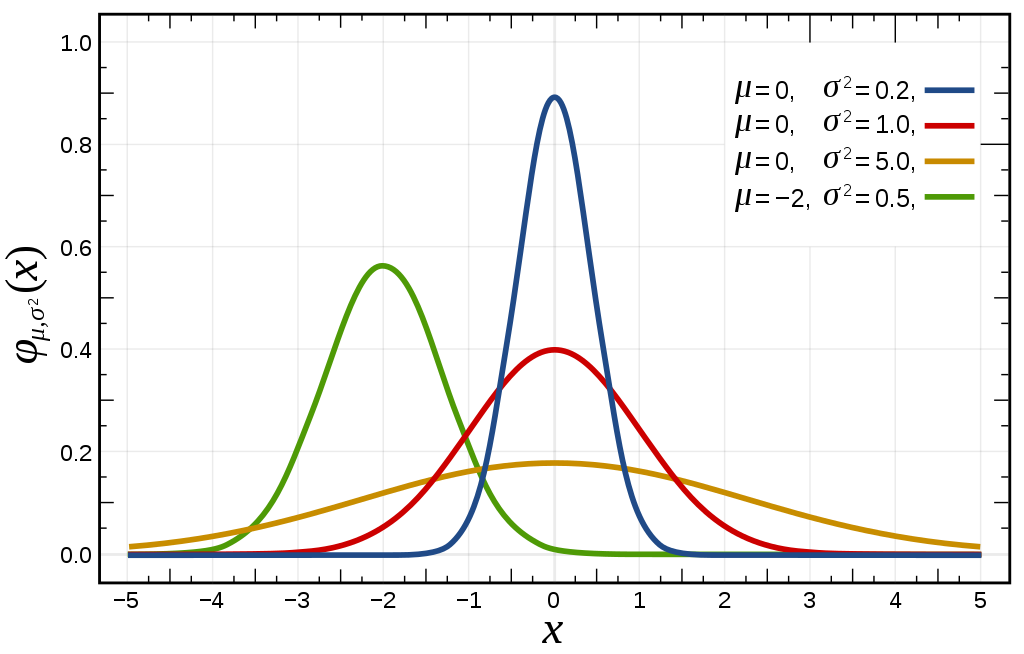
\includegraphics[width=0.4\textwidth, angle=-0]{1024px-norm.png}	
	\caption{Probability Density Function} 
	\label{fig_mom0}%
\end{figure}

\begin{figure}
	\centering 
	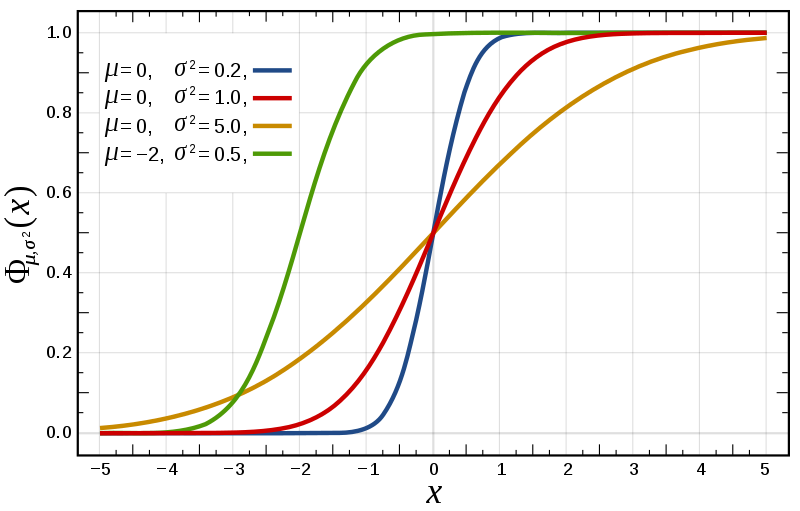
\includegraphics[width=0.4\textwidth, angle=-0]{800px-dist.png}	
	\caption{Physics Letters B journal cover} 
	\label{fig_mom0}%
\end{figure}

\subsection{Soft Gamma Ray Bursts}

Soft Gamma Repeaters are Neutron Stars called Magnetars. Magnetars have an extraordinarily strong magnetic field ranging from 101 4 to 101 5. Contrary to their name Soft Gamma Repeaters emit large amounts of energy number. Only when compared to a Gamma Ray Burst do Soft Gamma Repeaters seem dim. When these Neutron stars experience an (starquake) they produce a strong emmision of energy. Starquakes are simmilar to that of an earth quake on earth. This is what satellites see as a Soft Gamma Repeater. Satellite reading will show a pulsation in gamma readings. The neutron star itself isn’t pulsing.  After the initial eruption the energy disapates. When this is combined with the quick rotational period of magnatars it creates a light house efffect. In my model I used the euation represented below to model soft gamma repeaters. AMP is the aplitude of the soft gamma repeater. f is the frequency or the rotational period. t is the start time or the time which the first soft gamma repeater apeared. $t_1$ is the current time. 

\subsection{X-ray pulsars}

X-ray pulsars are formed because of the acceleration and (coliding) of matter at the poles of the neutron star. The poles of the netoron star rotate around an axis. We see neutron star only when the poles are pointed tword earth. Since to oples move twards and away form earth in a circle it looks like it is puling from earths point of view. In order to model this I used the equation below it is simmilar to the equation show in Neutron stars however it does not have a rate of decay. The burst on a soft gamma reapeater only last for a short period of time with larger burst lasting (several minutes). X-ray pulasrs last for (around 10,000 years)(sitation). The time scale of my model is only 1 year makeing it unresonable to add a rate of decay to the X-ray pulsars observed in my model. 

X
Are binary star systems.

A random equation, the Toomre stability criterion:

\subsection{X-ray Bursters}

X-ray bursters occur when a neutron star accreats matter on the surface of the star causing the surface of the star to explode. This additional matter is usualy acreated form a companion donner star. Thies star orbit around eachoter sloly matter is tranfered form the donner star to the Neutron star. This matter forms an acreation disk around the center of the star.
In my model I show these stars as already apearing in the night sky. (As steady X-ray stars that sudenly burst) The burst happens randomly however thier is a correlation between how large the last burst was and when the next burst will occur. This is because the larger the burst mas the more energy(feul) it burned and the more time it will take to accumalate fuel back to the state it once was in. In my model I accomplish this by multiplying the amplitude of the burst times a random number to determine the time in which the next burst will happen. 

\subsection{Model of Sky in Optical Light}
My model shows the view of the galaxy from earth using the galactic coordinate system. In the galatic coordinate system the center of the milky way is the center of the map. the majority of the stars are along the center of the map where the milky way is.(0 longitute) The stars which are futher from this center are stars that are closer to earth or bright object out side the milky way galaxy.
\begin{equation}
    Q = \frac{\sigma_v \times \kappa}{\pi \times G \times \Sigma}
\end{equation}

\section{Results}
%%\label{}
\lipsum[2]

\subsection{Subsection title}
\lipsum[3]

\begin{table}
\begin{tabular}{l c c c} 
 \hline
 Source & RA (J2000) & DEC (J2000) & $V_{\rm sys}$ \\ 
        & [h,m,s]    & [o,','']    & \kms          \\
 \hline
 NGC\,253 & 	00:47:33.120 & -25:17:17.59 & $235 \pm 1$ \\ 
 M\,82 & 09:55:52.725, & +69:40:45.78 & $269 \pm 2$ 	 \\ 
 \hline
\end{tabular}
\caption{Random table with galaxies coordinates and velocities, Number the tables consecutively in
accordance with their appearance in the text and place any table notes below the table body. Please avoid using vertical rules and shading in table cells.
}
\label{Table1}
\end{table}


\section{Discussion/Results}
%%\label{}
\lipsum[4]

\section{Summary and conclusions}
%%\label{}
\subsection{Succsuss}
\subsection{Limitations}
\subsection{Futurework}

\section{References}
All my references have 

\section*{Acknowledgements}
Thanks to ...

%% The Appendices part is started with the command \appendix;
%% appendix sections are then done as normal sections
\appendix

\section{Appendix title 1}
%% \label{}

\section{Appendix title 2}
%% \label{}

%% If you have bibdatabase file and want bibtex to generate the
%% bibitems, please use
%%
\bibliographystyle{elsarticle-harv} 
\bibliography{example}

%% else use the following coding to input the bibitems directly in the
%% TeX file.

%%\begin{thebibliography}{00}

%% \bibitem[Author(year)]{label}
%% For example:

%% \bibitem[Aladro et al.(2015)]{Aladro15} Aladro, R., Martín, S., Riquelme, D., et al. 2015, \aas, 579, A101


%%\end{thebibliography}

\end{document}

\endinput
%%
%% End of file `elsarticle-template-harv.tex'.
